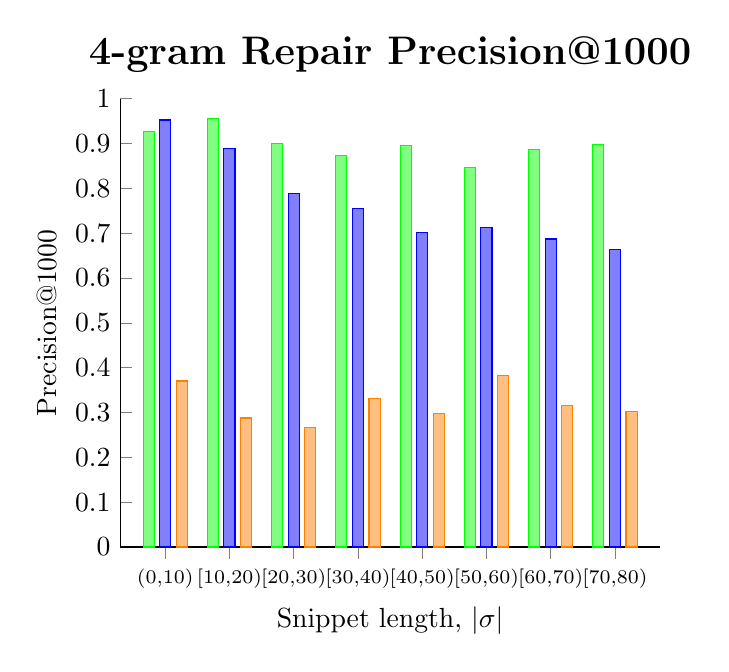
\begin{tikzpicture}
  \begin{axis}[
  xlabel={Snippet length, $|\sigma|$},
  ylabel={Precision@1000},
  title={\Large\textbf{4-gram Repair Precision@1000}},
  ybar,
  axis lines*=left,
  xtick={0, 10, 20, 30, 40, 50, 60, 70},
  ytick={0, 0.1, 0.2, 0.3, 0.4, 0.5, 0.6, 0.7, 0.8, 0.9, 1.0},
  xticklabels={{(}0{,}10{)}, {[}10{,}20{)}, {[}20{,}30{)}, {[}30{,}40{)}, {[}40{,}50{)}, {[}50{,}60{)}, {[}60{,}70{)}, {[}70{,}80{)}},
  x tick label style={font=\scriptsize},
  ymax=1.0,
  ymin=0.0,
  bar width=4pt,
  ]
  \addplot[green, fill=green!50] coordinates { (0, 0.9276315789473685) (10, 0.9565217391304348) (20, 0.9010238907849829) (30, 0.8724137931034482) (40, 0.8961937716262975) (50, 0.8472222222222222) (60, 0.8875) (70, 0.8977272727272727) };
  \addplot[blue, fill=blue!50] coordinates { (0, 0.9523809523809523) (10, 0.8896321070234113) (20, 0.7889273356401384) (30, 0.754325259515571) (40, 0.702054794520548) (50, 0.7128712871287128) (60, 0.6870748299319728) (70, 0.6636363636363637) };
  \addplot[orange, fill=orange!50] coordinates { (0, 0.37037037037037035) (10, 0.2876712328767123) (20, 0.26666666666666666) (30, 0.33116883116883117) (40, 0.2982456140350877) (50, 0.38333333333333336) (60, 0.3157894736842105) (70, 0.30158730158730157) };
  \end{axis}
\end{tikzpicture}